\documentclass{article}
\usepackage{graphicx}
\usepackage[style=ieee]{biblatex} % Establecer el estilo de las referencias como IEEE
\usepackage{xcolor}
\usepackage{hyperref}
\usepackage{titletoc}
\usepackage{adjustbox}

\hypersetup{
    colorlinks=true,
    linkcolor=blue, % Color del texto del enlace
    urlcolor=blue % Color del enlace
}

\usepackage{longtable} % Agrega el paquete longtable

\definecolor{mygreen}{RGB}{0,128,0}

\usepackage{array} % Para personalizar la tabla
\usepackage{booktabs} % Para líneas horizontales de mejor calidad
\usepackage{graphicx} % Paquete para incluir imágenes
\usepackage{float}

% Definir márgenes
\usepackage[margin=1in]{geometry}

\renewcommand{\contentsname}{\textcolor{mygreen}{Tabla de Contenidos}}

\begin{document}

\begin{titlepage}
    \centering
    % Logo de la Universidad
    
\includegraphics[width=0.48\textwidth]{logo_universidad.png}
    \par\vspace{2cm}

    % Nombre de la Universidad y detalles del curso
    {\Large \textbf{Universidad Nacional de Colombia} \par}
    \vspace{0.5cm}
    {\large Ingeniería de Sistemas y Computación \par}
    {\large 2025969 Modelos estocásticos y simulación en computación y comunicaciones (01)\par}
    \vspace{3cm}

    % Detalles del laboratorio y actividad
    {\large \textbf{Taller 1} \par}
    {\large Taller 1 \par}
    \vspace{3cm}

    % Lista de integrantes
    {\large \textbf{Integrantes:} \par}
    \vspace{0.5cm}
    \begin{tabular}{ll}
    Javier Andrés Tarazona Jiménez & jtarazonaj@unal.edu.co \\
    Jefferson Duvan Ramirez Castañeda & jeramirezca@unal.edu.co \\
    Yenifer Yulieth Mora Segura & ymoras@unal.edu.co \\
    Javier Carrillo & @unal.edu.co \\
    Grevy Joner Rincon Mejia & grrinconm@unal.edu.co \\
    Esteban Carranza & jcarranza@unal.edu.co \\
    Diego & @unal.edu.co \\
    \end{tabular}
    \par\vspace{3cm}

    % Fecha
    {\large Junio 7 de 2025 \par}
\end{titlepage}

\tableofcontents % Inserta la tabla de contenidos

\newpage % Salto de página para separar la tabla de contenidos del contenido del documento

% Contenido del artículo----------------------------------------------------------

%---------------------------------------------------------------------------------
% Intro --------------------------------------------------------------------------
%---------------------------------------------------------------------------------

\section{Introducción}\label{sec:intr}

En un escenario de extinción de incendios forestales mediante drones cooperativos, la comunicación inalámbrica entre los dispositivos se ve constantemente afectada por obstáculos naturales (árboles, relieve), interferencias y la movilidad dinámica del enjambre. Este trabajo aborda un problema concreto: cuando un dron se desconecta momentáneamente del líder de su grupo (Cluster Head) debido a estas adversidades, pierde capacidad de coordinación crítica para la misión, retrasando la respuesta ante focos de incendio y aumentando el consumo energético por retransmisiones.

Para resolver este desafío operativo, proponemos una solución basada en redes MANET jerárquicas, donde los drones desconectados adoptan temporalmente el rol de líder (CH-temporal). Este enfoque práctico se sustenta en modelos teóricos de movilidad grupal y algoritmos de reclusterización dinámica, evaluando umbrales de desconexión basados en calidad de señal, energía remanente y presencia de obstáculos. La implementación en NS-3 demuestra que este método reduce el tiempo de recuperación de conexiones comparado con protocolos tradicionales, manteniendo la efectividad del enjambre incluso en condiciones adversas.


%---------------------------------------------------------------------------------
% Marco Teórico ------------------------------------------------------------------
%---------------------------------------------------------------------------------

\section{Marco Teórico}\label{sec:marc}

\section{Descripción y Justificación del Problema a Resolver}\label{sec:descr}


\subsection{Objetivo Principal}

%---------------------------------------------------------------------------------
% Diseño de la solución ---------------------------------------------------------
%---------------------------------------------------------------------------------



\section{Diseño de la solución}

La solución desarrollada está basada en el modelo de comportamiento de Boids para simular la movilidad de nodos en una red ad hoc. Este modelo adapta las reglas clásicas de \textit{cohesión}, \textit{alineación} y \textit{separación}, incorporando elementos adicionales como nodos líderes, mecanismos de selección dinámica de líderes mediante el algoritmo de clustering ponderado (WCA), interacción con eventos externos (como incendios) y una infraestructura de comunicación entre nodos basada en enlaces bidireccionales.

\subsection{Metodología}

El desarrollo siguió un enfoque incremental. Inicialmente se construyó la jerarquía básica de nodos (líderes y seguidores), luego se integró la lógica de comportamiento y movilidad basada en el modelo Boids. Posteriormente se añadieron componentes estocásticos y eventos del entorno, como focos de incendio. Finalmente, se realizaron múltiples simulaciones para evaluar el rendimiento del modelo frente a distintos escenarios y configuraciones.

\subsection{Estructura general del sistema}

El sistema está compuesto por los siguientes módulos principales:

\begin{itemize}
    \item \textbf{BoidsMobilityModel}: clase que extiende el modelo de movilidad de NS-3 y contiene la lógica del comportamiento individual de cada nodo.
    \item \textbf{Gestor de líderes}: módulo encargado de la asignación inicial de líderes y del recálculo dinámico basado en WCA.
    \item \textbf{Módulo de eventos externos}: introduce elementos del entorno como incendios que influyen en el comportamiento de los nodos líderes.
    \item \textbf{Sistema de comunicación}: permite el intercambio de mensajes entre nodos vecinos, facilitando la detección de líderes, el seguimiento de objetivos y la formación de clusters.
\end{itemize}

\subsection{Reglas de comportamiento Boid}

Cada nodo se comporta como un Boid y actualiza su posición en función de su rol y de las siguientes reglas:

\begin{itemize}
    \item \textbf{Separación:} evita la colisión entre nodos manteniendo una distancia mínima entre vecinos cercanos.
    
    \item \textbf{Alineación:} los seguidores adaptan su dirección en función de la velocidad promedio de sus vecinos más cercanos.
    
    \item \textbf{Cohesión:} los seguidores buscan mantenerse próximos a su líder si se encuentra dentro del radio de cohesión definido.
    
    \item \textbf{Atracción hacia objetivos:} los líderes se orientan hacia eventos externos (como focos de incendio) ubicados dentro de su radio de influencia.
\end{itemize}

\subsection{Liderazgo dinámico y algoritmo WCA}

Cada nodo puede desempeñar el rol de líder o seguidor. Al inicio de la simulación, se asignan aleatoriamente los roles. A los líderes se les asigna un objetivo dentro del área de simulación, el cual puede cambiar en respuesta a eventos externos.

Si un nodo seguidor se encuentra aislado, es decir, sin un líder en su radio de cohesión, evalúa su potencial de liderazgo utilizando el algoritmo \textit{WCA} (Weighted Clustering Algorithm). Este algoritmo considera múltiples factores que se normalizan para obtener un puntaje de liderazgo (\texttt{WCA\_Score}):

\begin{itemize}
    \item \textit{Energía residual} (\(E\)): porcentaje de energía restante del nodo, normalizada en el rango \([0,1]\).
    \item \textit{Grado de conectividad} (\(D\)): número de vecinos directos, normalizado respecto a un máximo teórico de 10.
    \item \textit{Distancia a objetivos} (\(T\)): inversa de la distancia promedio del nodo a los objetivos activos, normalizada considerando un rango de hasta 200 metros.
    \item \textit{Movilidad} (\(M\)): estabilidad del nodo, calculada como la inversa de su velocidad actual, con una velocidad máxima de 10 m/s.
\end{itemize}

El cálculo del puntaje se define como:

\[
{WCA\_Score} = w_1 \cdot E + w_2 \cdot D + w_3 \cdot T + w_4 \cdot M
\]
donde los pesos utilizados son:

\[
w_1 = 0.4, \quad w_2 = 0.3, \quad w_3 = 0.2, \quad w_4 = 0.1
\]

El resultado se limita al rango \([0, 1]\) mediante:

\[
{WCA\_Score} = \max\left(0,\ \min\left(1,\ {WCA\_Score}\right)\right)
\]

El nodo aislado con el mayor \texttt{WCA\_Score} se autonombrará líder en ausencia de otros líderes cercanos.

\subsection{Espacio de simulación y condiciones de frontera}

La simulación se desarrolla en un área de $1000 \times 1000$ unidades. Se implementa una condición de frontera toroidal (\textit{wrapping}), permitiendo que los nodos que salen por un borde reaparezcan por el lado opuesto. Esto evita acumulaciones artificiales y simula un entorno continuo sin bordes rígidos.

\subsection{Actualización de posiciones}

Cada nodo actualiza su posición en intervalos regulares de tiempo, considerando sus vectores de dirección y las fuerzas derivadas de las reglas del modelo Boid. Se aplican límites a la velocidad y se normalizan las direcciones para evitar aceleraciones bruscas o inmovilización de nodos.

\subsection{Visualización y exportación de datos}

Al finalizar cada simulación, se exportan datos relevantes a archivos de salida, incluyendo las posiciones de los nodos, los roles asignados (líder o seguidor), las trayectorias seguidas por cada nodo y la ubicación de eventos externos, como los incendios.
Esta información permite un análisis post-simulación de métricas clave como cobertura, tiempo de respuesta o efectividad en la extinción de eventos.

\subsection{Configurabilidad del modelo}

La clase \texttt{BoidsMobilityModel} incluye métodos \texttt{Set} que permiten ajustar los parámetros más relevantes del comportamiento de los nodos, tales como el radio de cohesión de los seguidores, el radio de influencia de los líderes, la velocidad máxima de los nodos, la frecuencia de actualización de posición, la inicialización del rol de los nodos (porcentaje de líderes), y parámetros del algoritmo WCA como pesos y umbrales de energía o distancia. 

En la Figura~\ref{fig:uml-boids} se presenta el diagrama UML de la clase \texttt{BoidsMobilityModel}, donde se observan sus atributos principales, métodos de configuración, y lógica asociada al liderazgo y simulación de incendios.

\begin{figure}[H]
    \centering
    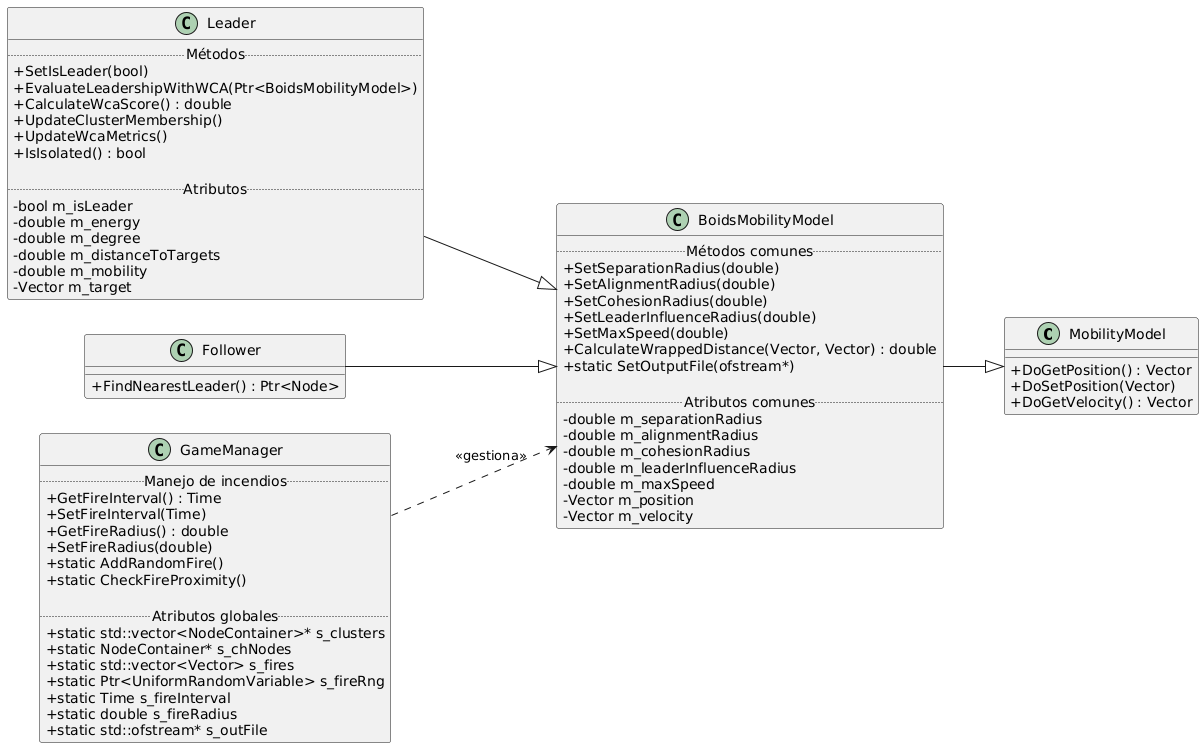
\includegraphics[width=0.9\textwidth]{class_diagram.png}
    \caption{Diagrama UML de la clase \texttt{BoidsMobilityModel}.}
    \label{fig:uml-boids}
\end{figure}



\section{Código Fuente}\label{sec:cod}

El código fuente completo de este modelo se encuentra adjunto en el buzón 
(06 Tarazona Jimenez Javier Andres 02.zip)
y disponible en el repositorio GitHub del proyecto:

\begin{center}
\url{https://github.com/JavierTarazona06/ME01_Tareas/tree/main/Tarea06/Code}
\end{center}

El repositorio contiene:
\begin{itemize}
\item Los módulos principales para generación de datos (\texttt{generator.py})
\item Implementación del algoritmo PBS (\texttt{toolsStats.py})
\item Scripts de simulación para los 4 escenarios, ejecutables desde (\texttt{main.py})
\item Archivo program.py de para la definición de las constantes del programa 
    (\texttt{constants\_program.py})
\item Archivo de métricas (\texttt{metrics.py})
\end{itemize}

%---------------------------------------------------------------------------------
% Manual Usuario ---------------------------------------------------------
%---------------------------------------------------------------------------------

\section{Manual Usuario}\label{sec:man_u}


%---------------------------------------------------------------------------------
% Manual Técnico ---------------------------------------------------------
%---------------------------------------------------------------------------------

\section{Manual Técnico}\label{sec:man_t}



\section{Experimentación}\label{sec:exp}

\subsection{Documentación}


\subsection{Escenario 1:}


\subsection{Escenario 2:}

\subsection{Escenario 3:}

\subsection{Comparación resultados}

%---------------------------------------------------------------------------------
% Conclusiones ---------------------------------------------------------
%---------------------------------------------------------------------------------

\section{Conclusiones}\label{sec:concl}

La integración del modelo Boids permite simular comportamientos realistas en redes móviles
El uso del modelo Boids reproduce dinámicas naturales de agrupamiento, separación y alineación, lo cual resulta útil para representar redes MANET (redes móviles ad hoc) en situaciones como búsqueda, exploración o evacuación.
%---------------------------------------------------------------------------------
% Recomendaciones ---------------------------------------------------------
%---------------------------------------------------------------------------------

\section{Recomendaciones}\label{secrecomen}

Aunque el movimiento fue simulado correctamente, se recomienda analizar también cómo este afecta la calidad de las comunicaciones (ej. transmisión de datos entre nodos), especialmente al estar en constante movimiento y ante interrupciones externas.

\section{Referencias}
\renewcommand{\refname}{}
\begin{thebibliography}{9}

\bibitem{ref} \label{ref:BPS} M. Bichler, S. Merting, and A. Uzunoglu, 
“Assigning Course Schedules: About Preference Elicitation, Fairness, and Truthfulness,” 
arXiv preprint arXiv:1812.02630, 2018. [En línea]. Disponible en: 
\url{https://arxiv.org/abs/1812.02630}



\end{thebibliography}

\end{document}